\documentclass[12pt]{article}
\usepackage[a3paper]{geometry}
\usepackage[utf8]{inputenc}
\usepackage{tikz}
\usetikzlibrary{automata, positioning, arrows, shapes.geometric}

\tikzstyle{startstop} = [rectangle, rounded corners, minimum width=3cm, minimum height=1cm,text centered, draw=black, fill=red!30]
\tikzstyle{io} = [trapezium, trapezium left angle=70, trapezium right angle=110, minimum width=3cm, minimum height=1cm, text centered, draw=black, fill=blue!30]
\tikzstyle{process} = [rectangle, minimum width=3cm, minimum height=1cm, text centered, draw=black, fill=orange!30]
\tikzstyle{decision} = [diamond, minimum width=3cm, minimum height=1cm, text centered, draw=black, fill=green!30]
\tikzstyle{arrow} = [thick,->,>=stealth]
\title{Compiler Lexer DFA}
\author{hiterzmy }
\date{April 2019}

\begin{document}
% \begin{figure}[htb]
%     \centering
%     \begin{tikzpicture}[->,>=stealth',shorten >=1pt,auto,node distance=2.8cm,semithick]
%     \node[state, initial] (q2) {$2$};
%     \node[state, right of=q2] (q3) {$3$};
%     \node[state, right of=q3] (q4) {$4$};
%     \node[state, right of=q4] (q5) {$5$};
%     \node[state, right of=q5] (q6) {$6$};
%     \node[state, right of=q6] (q7) {$7$};
%     \node[state, right of=q7] (q8) {$8$};
%     \node[state, accepting, right of=q8] (q9) {$9$};
%     \node[state, above of=q3] (q12) {$12$};
%     \node[state, accepting, below of=q4] (q10) {$10$};
%     \node[state, accepting, below of=q7] (q11) {$11$};
%     \draw (q2) edge [above] node {digit} (q3)
%         (q3) edge [loop above] node {digit} (q3)
%         (q3) edge [above] node {\textbf{.}} (q4)
%         (q4) edge [above] node {digit} (q5)
%         (q5) edge [loop above] node {digit} (q5)
%         (q5) edge [above] node {E or e} (q6)
%         (q6) edge [above] node {+ or -} (q7)
%         (q7) edge [above] node {digit} (q8)
%         (q8) edge [loop above] node {digit} (q8)
%         (q8) edge [above] node {other} (q9)
%         (q3) edge [bend right, below] node {E or e} (q6)
%         (q6) edge [bend right, below] node {digit} (q8)
%         (q2) edge [bend left, above] node {\textbf{.}} (q12)
%         (q12) edge [bend left, above] node {digit} (q5)
%         (q3) edge [bend right, below] node {other} (q10)
%         (q5) edge [bend right, below] node {other} (q11)
%         (q4) edge [bend right, below] node {other} (q11);
%     \end{tikzpicture}
%     \caption{DFA of the numbers(\textbf{other} is char that not digit)}
%     \label{fig:number}
% \end{figure}

% \begin{figure}[htb]
%     \centering
%     \begin{tikzpicture}[->,>=stealth',shorten >=1pt,auto,node distance=3cm,semithick]
%     \node[state, initial] (q1) {$1$};
%     \node[state, right of=q1] (q2) {$2$};
%     \node[state, accepting, right of=q2] (q3) {$3$};
%     \draw (q1) edge [above] node{letter or '\_'} (q2)
%         (q2) edge [loop above] node {letter or digit or '\_'} (q2)
%         (q2) edge [above] node {other} (q3);
%     \end{tikzpicture}
%     \caption{DFA of the identifier\ (\textbf{other} is not letter, digit or '\_')}
%     \label{fig:id}
% \end{figure}

% \begin{figure}[htb]
%     \centering
%     \begin{tikzpicture}[->,>=stealth',shorten >=1pt,auto,node distance=3cm,semithick]
%     \node[state, initial] (q1) {$1$};
%     \node[state, right of=q1] (q2) {$2$};
%     \node[state, right of=q2] (q3) {$3$};
%     \node[state, right of=q3] (q4) {$4$};
%     \node[state, accepting, right of=q4] (q5) {$5$};
%     \draw (q1) edge [above] node {/} (q2)
%         (q2) edge [above] node {*} (q3)
%         (q3) edge [loop above] node {other} (q3)
%         (q3) edge [above] node {*} (q4)
%         (q4) edge [loop above] node {*} (q4)
%         (q4) edge [above] node {/} (q5)
%         (q4) edge [bend left, below] node {other} (q3);
%     \end{tikzpicture}
%     \caption{DFA of the comment\ (\textbf{other} is not letter, digit or '\_')}
%     \label{fig:comment}
% \end{figure}
\begin{center}
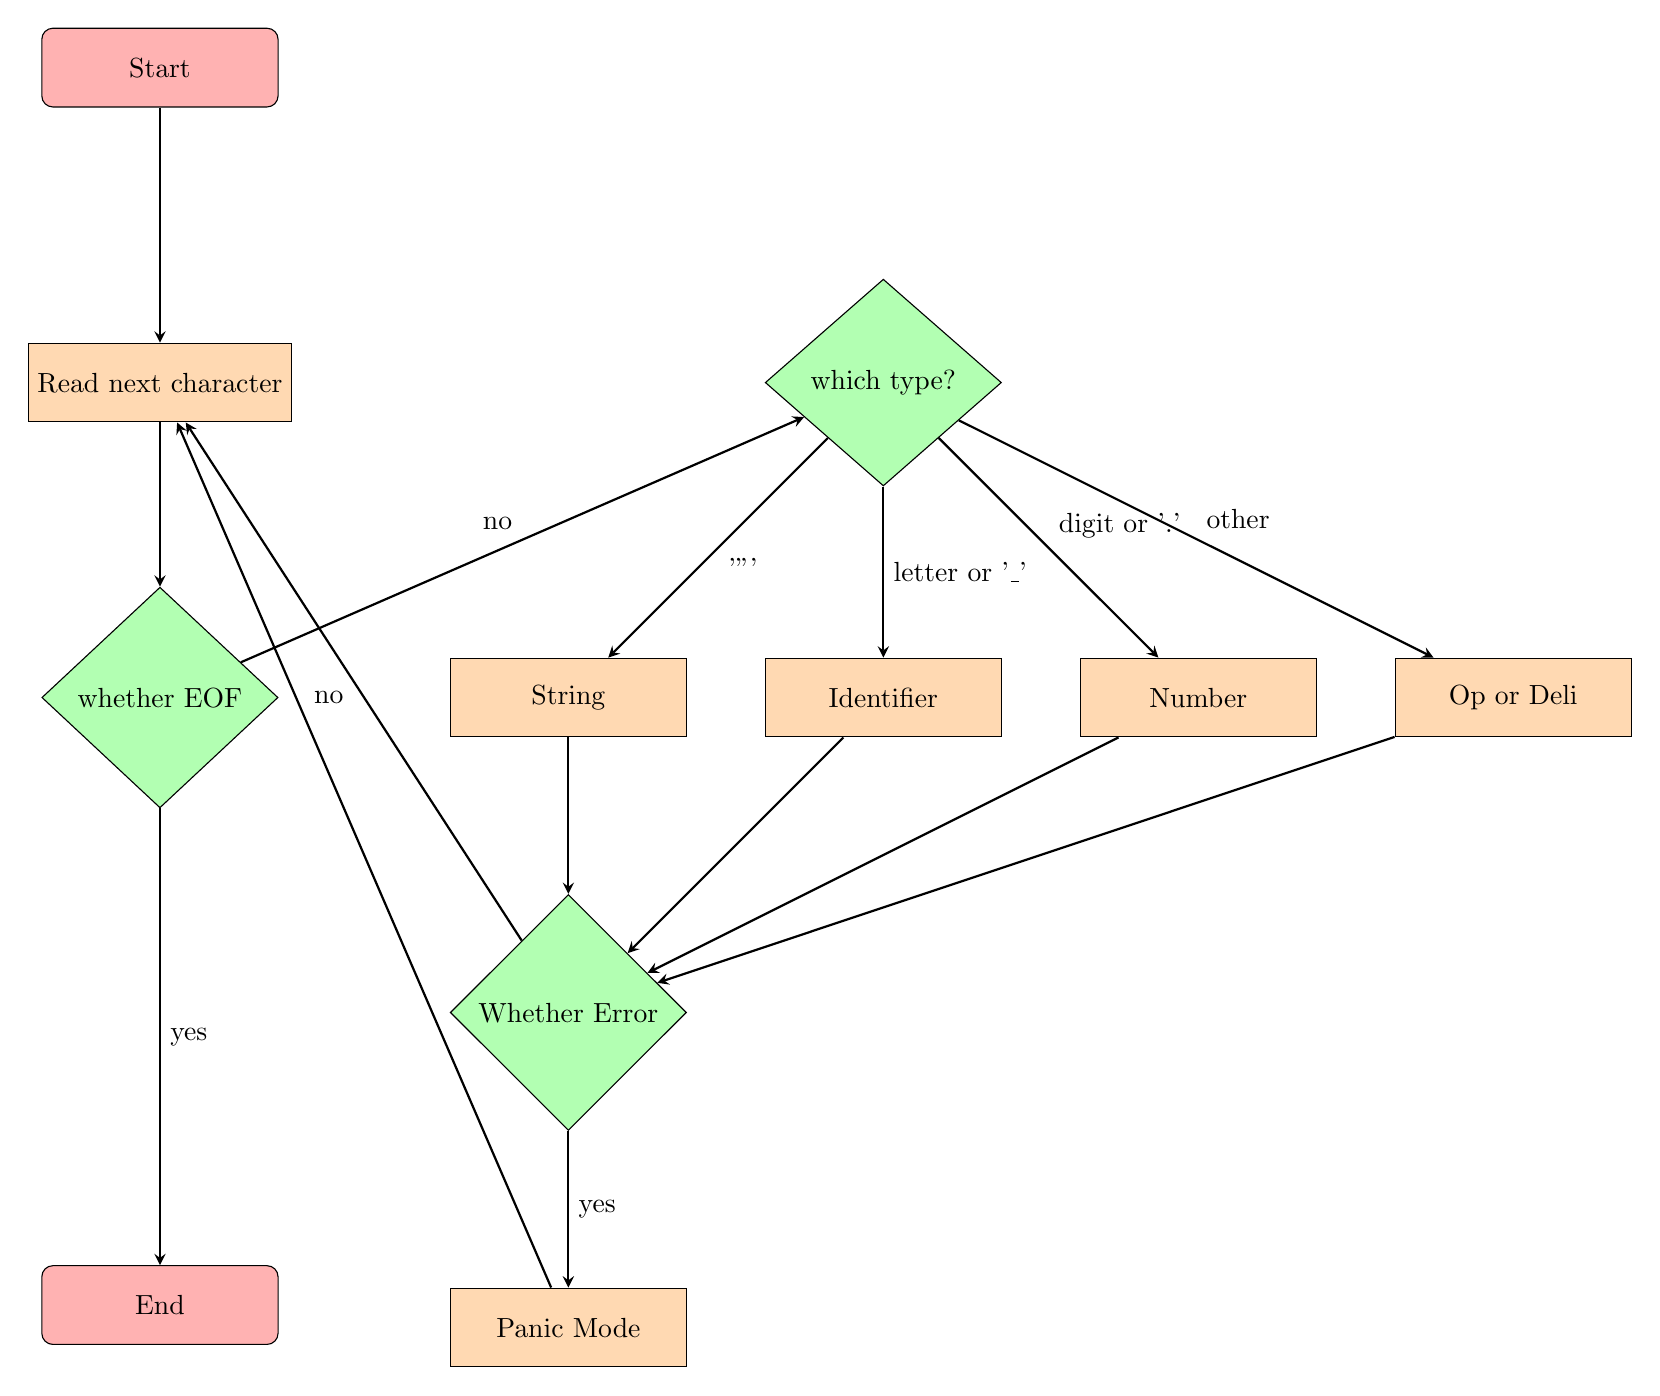
\begin{tikzpicture}[node distance=4cm]
\node (start) [startstop] {Start};
\node (input) [process, below of=start] {Read next character};
\node (eof) [decision, below of=input] {whether EOF};
\node (type_of_char) [decision, right=6cm of input] {which type?};
\node (id) [process, below of=type_of_char] {Identifier};
\node (number) [process, right of=id] {Number};
\node (string) [process, left of=id] {String};
\node (op) [process, right of=number] {Op or Deli};
\node (error) [decision, below of=string] {Whether Error};
\node (panic) [process, below of=error] {Panic Mode};
\draw [arrow] (start) -- (input);
\draw [arrow] (input) -- (eof);
\draw [arrow] (eof) -- node [auto] {no} (type_of_char);
\draw [arrow] (type_of_char) --node [auto] {digit or '.'} (number);
\draw [arrow] (type_of_char) --node [auto] {letter or '\_'} (id);
\draw [arrow] (type_of_char) --node [auto] {'"'} (string);
\draw [arrow] (type_of_char) --node [auto] {other} (op);
\draw [arrow] (id) -- (error);
\draw [arrow] (number) -- (error);
\draw [arrow] (op) -- (error);
\draw [arrow] (string) -- (error);
\draw [arrow] (error) --node [auto] {yes} (panic);
\draw [arrow] (error) -- node [auto] {no} (input);

\node (end) [startstop, below=5.8cm of eof] {End};
\draw [arrow] (eof) -- node [auto] {yes} (end);
\draw [arrow] (panic) -- (input);
\end{tikzpicture}
\end{center}

\end{document}
